\documentclass[UTF8,a4paper,12pt]{ctexart}
\usepackage[utf8]{inputenc}
\usepackage{amsmath}
\usepackage{pdfpages}
\usepackage{graphicx}
\usepackage{wrapfig}
\usepackage{listings}
\title{第一次仿真实验报告}
\author{张蔚桐\ 2015011493\ 自55}
\begin {document}
\maketitle
\section{}
\subsection{}
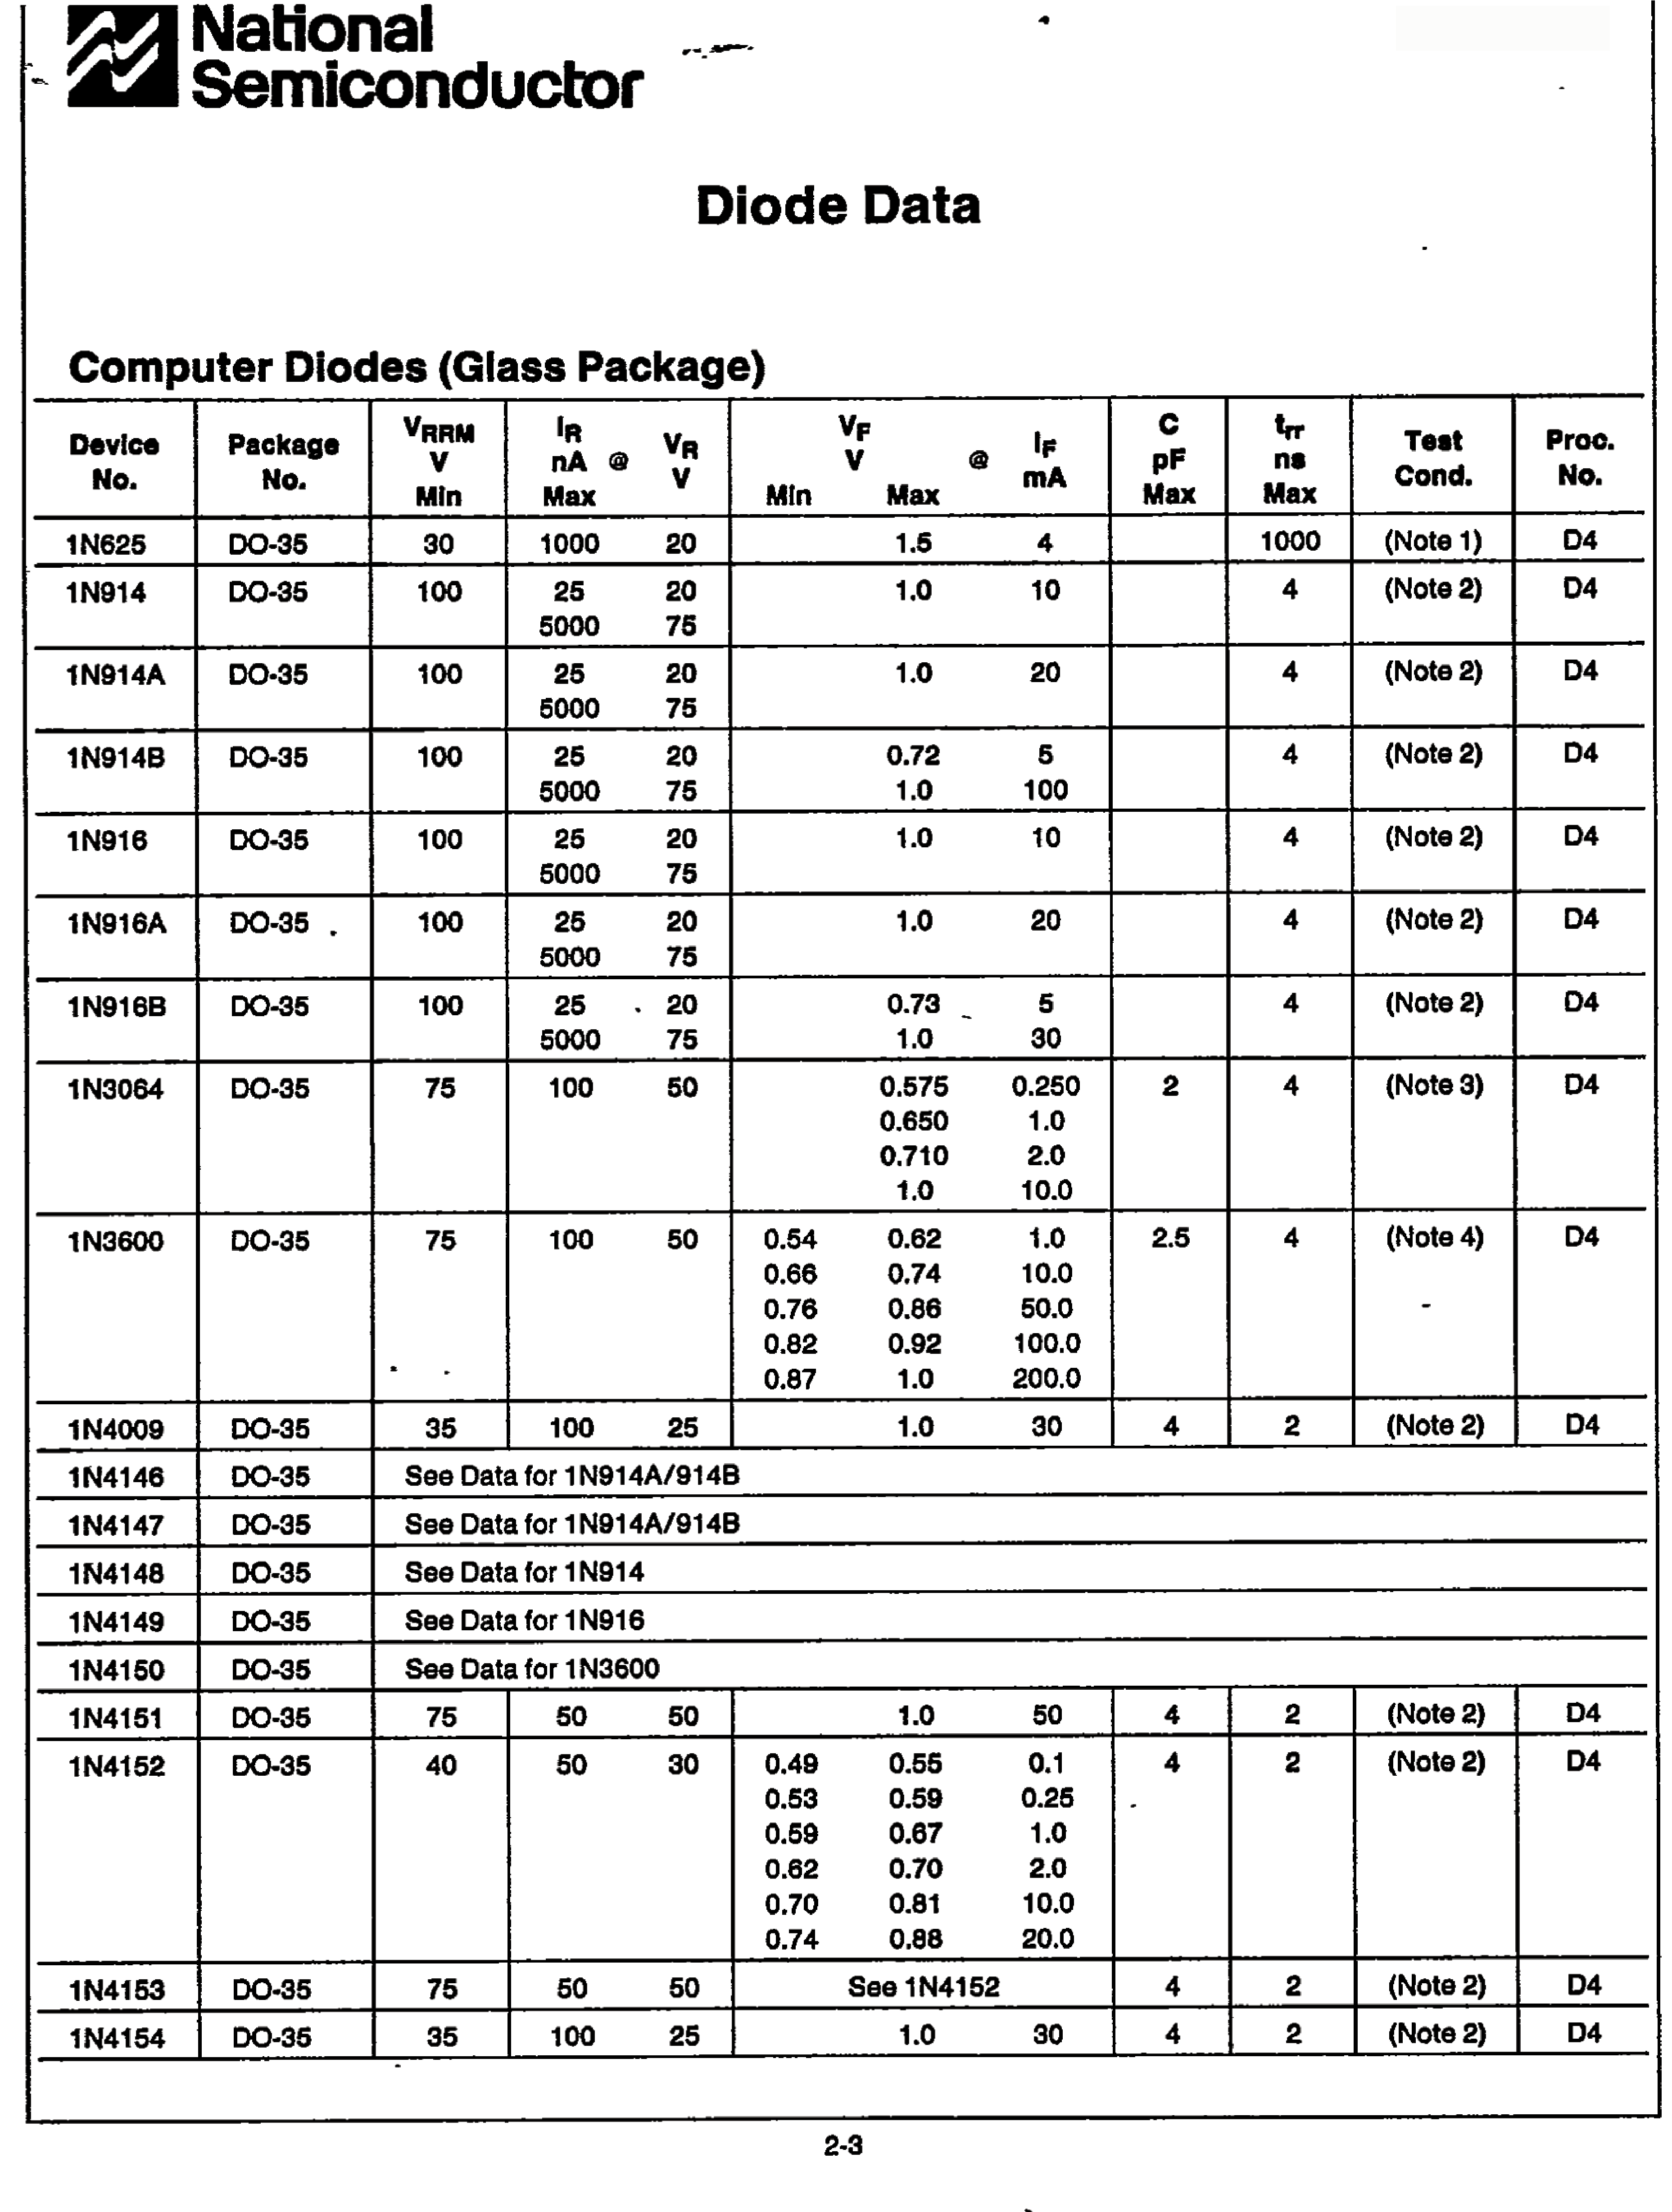
\includepdf[width=\textwidth]{datasheet1N3064.pdf}
\begin {wrapfigure}{r}{0pt}
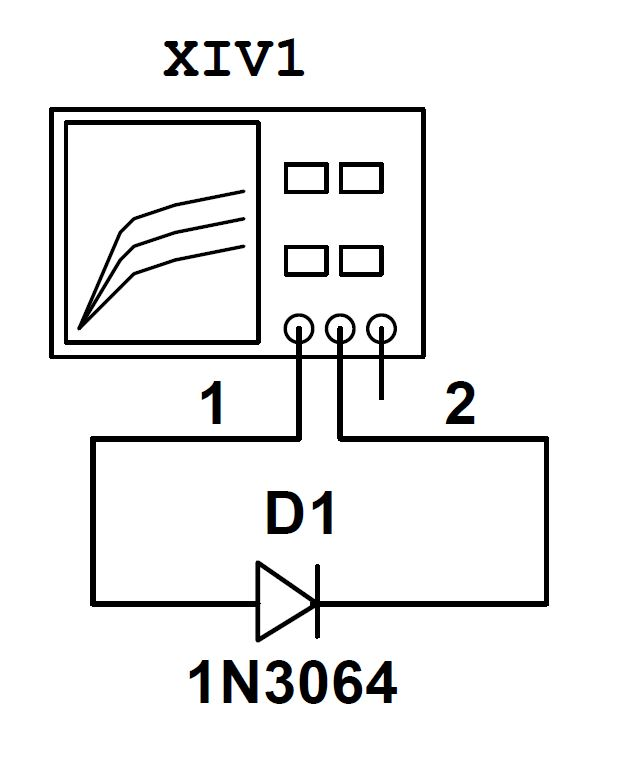
\includegraphics [width=40mm]{cap/8.JPG}
\end {wrapfigure}

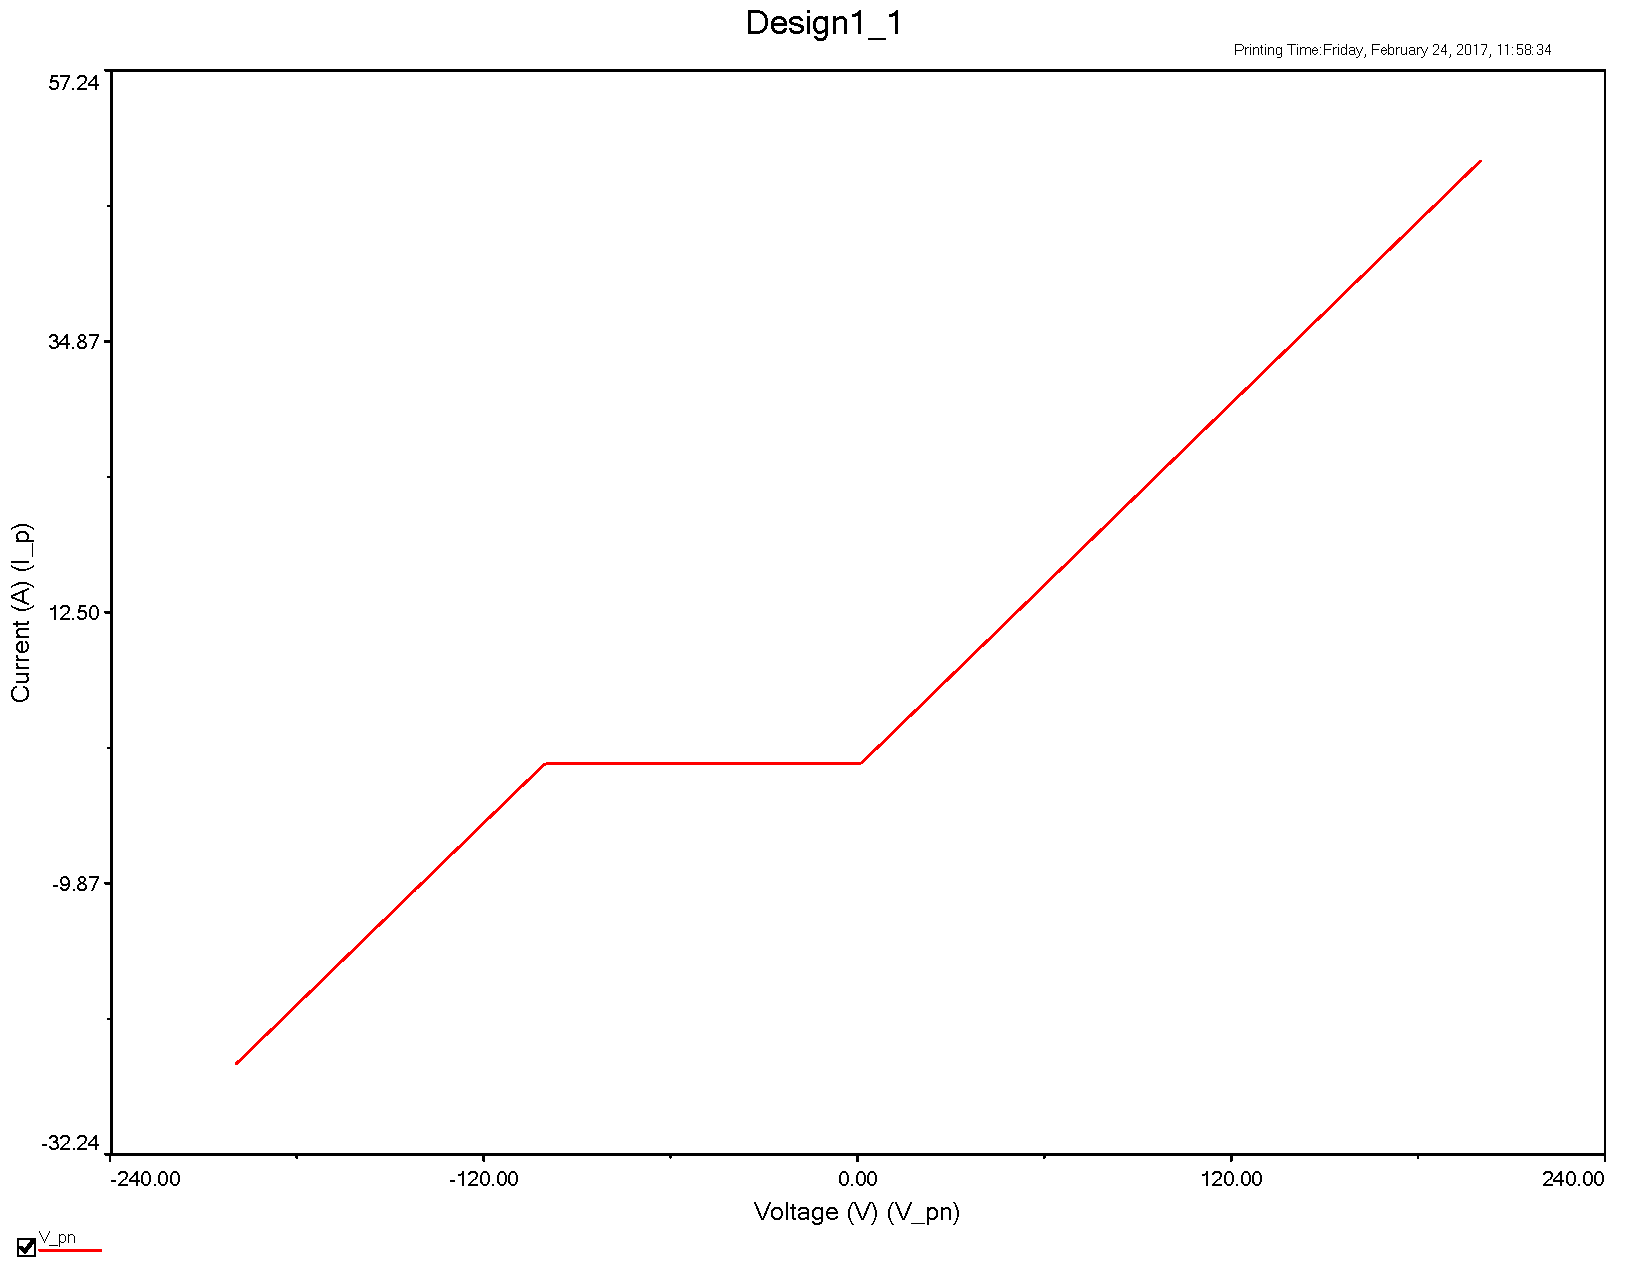
\includepdf[width=\textwidth]{general1D.pdf}
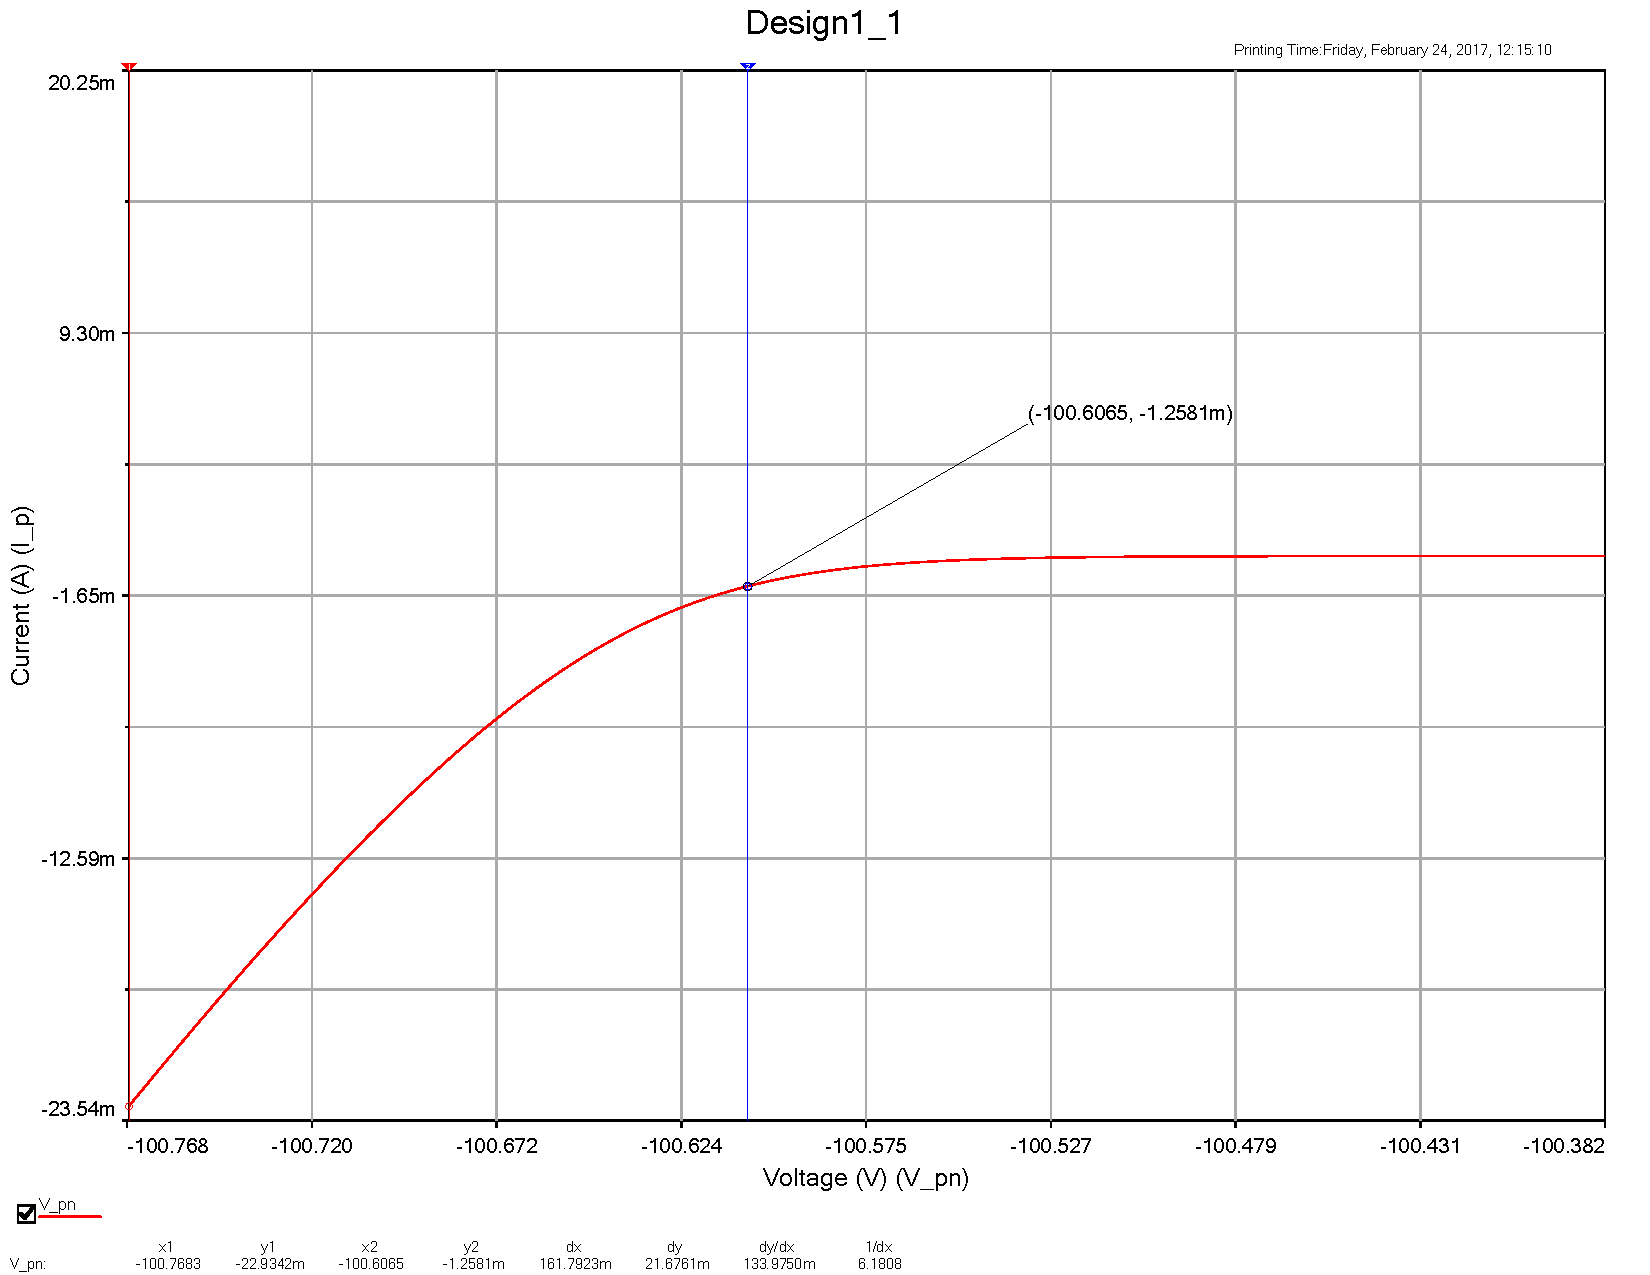
\includepdf[width=\textwidth]{efee.pdf}
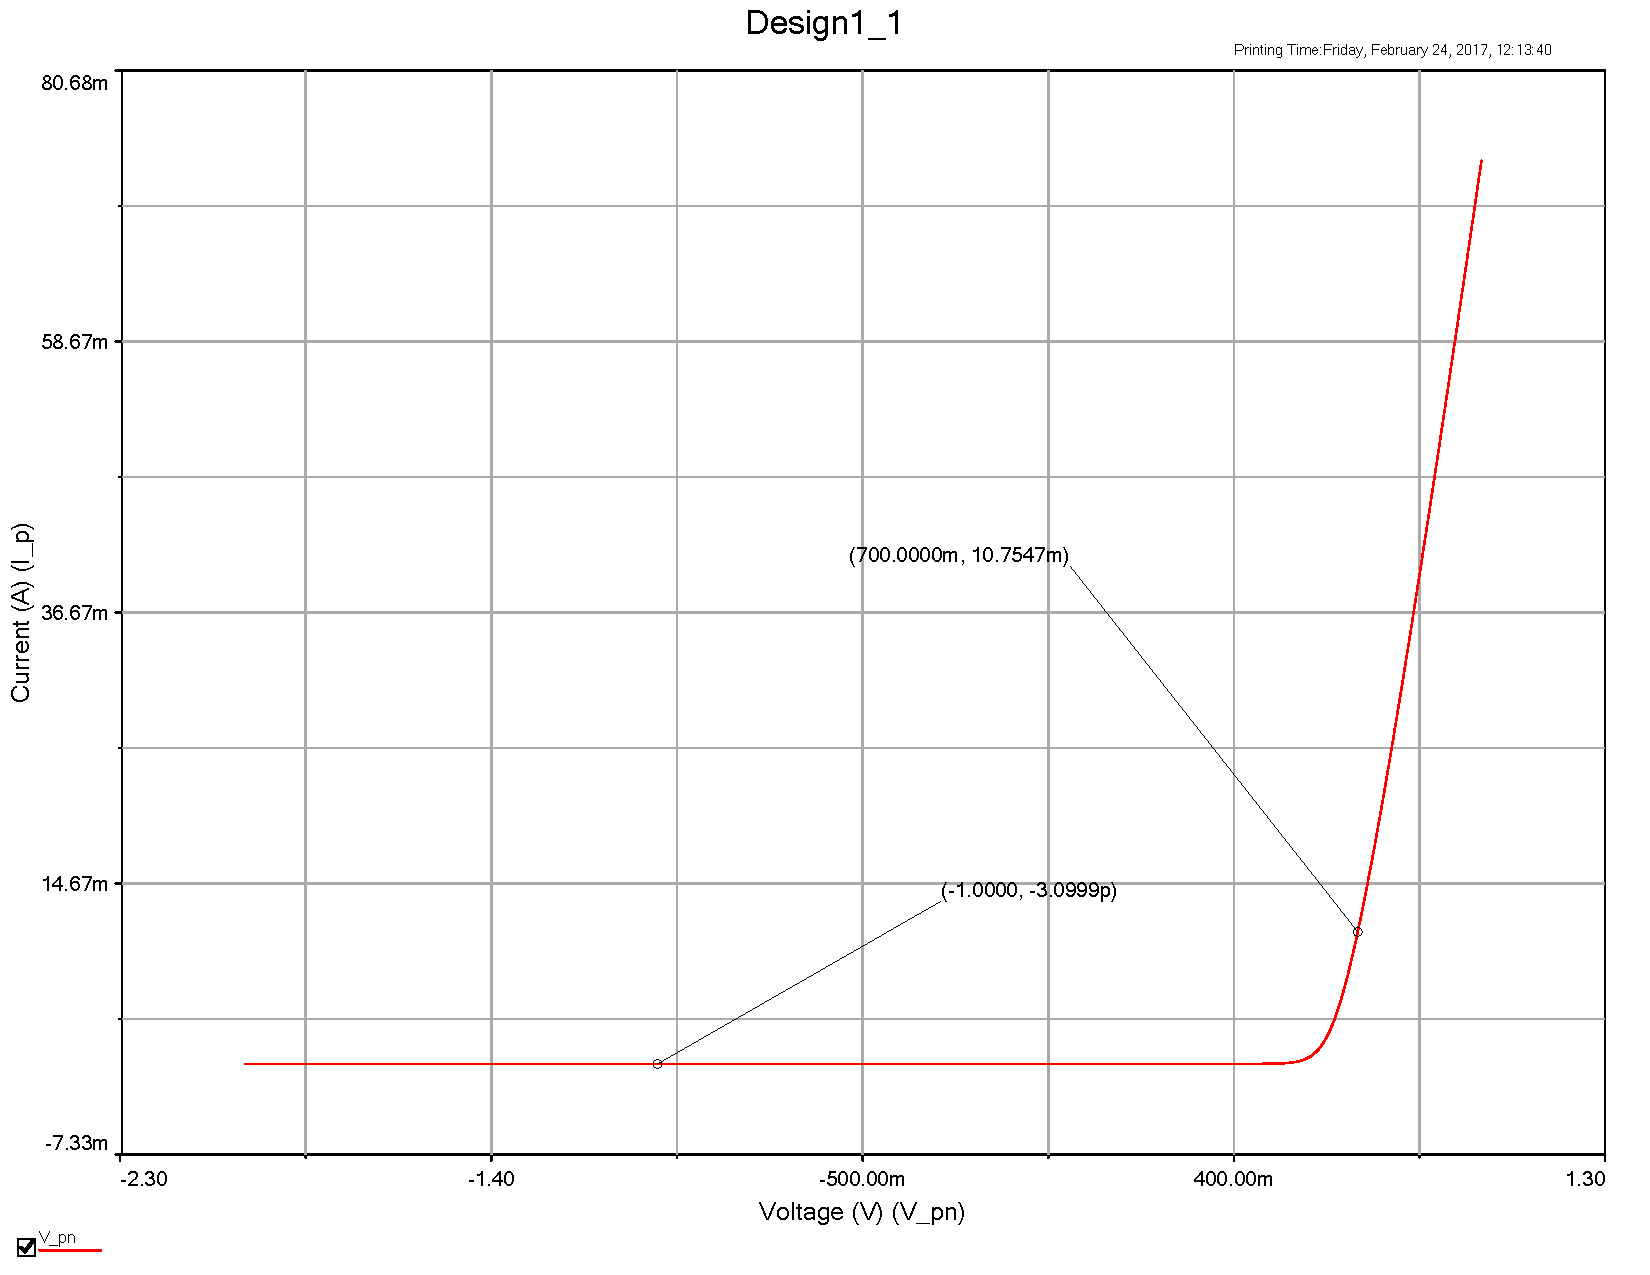
\includepdf[width=\textwidth]{fffe.pdf}


\subsection{}


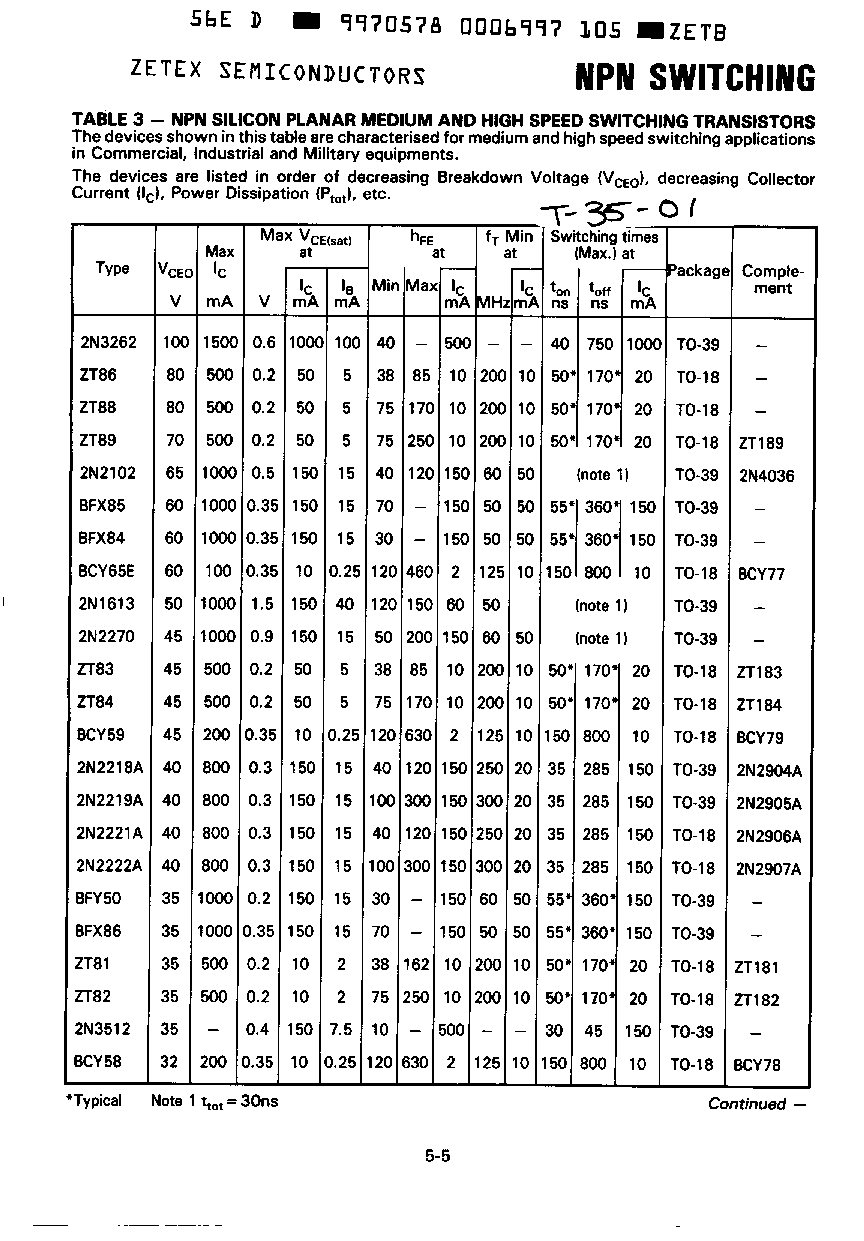
\includepdf[width=\textwidth]{ZETXS03326-1.pdf}
\begin {wrapfigure}{r}{0pt}
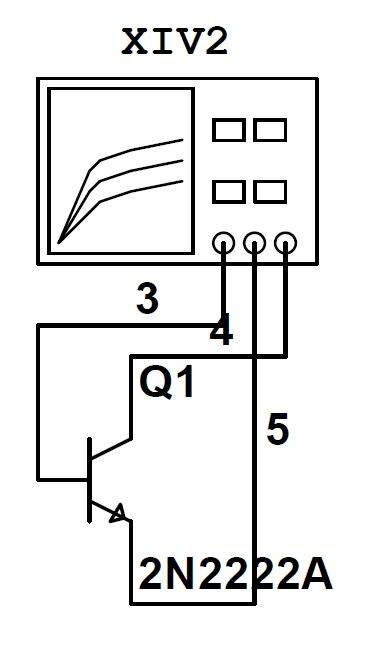
\includegraphics [width=40mm]{cap/9.JPG}
\end {wrapfigure}
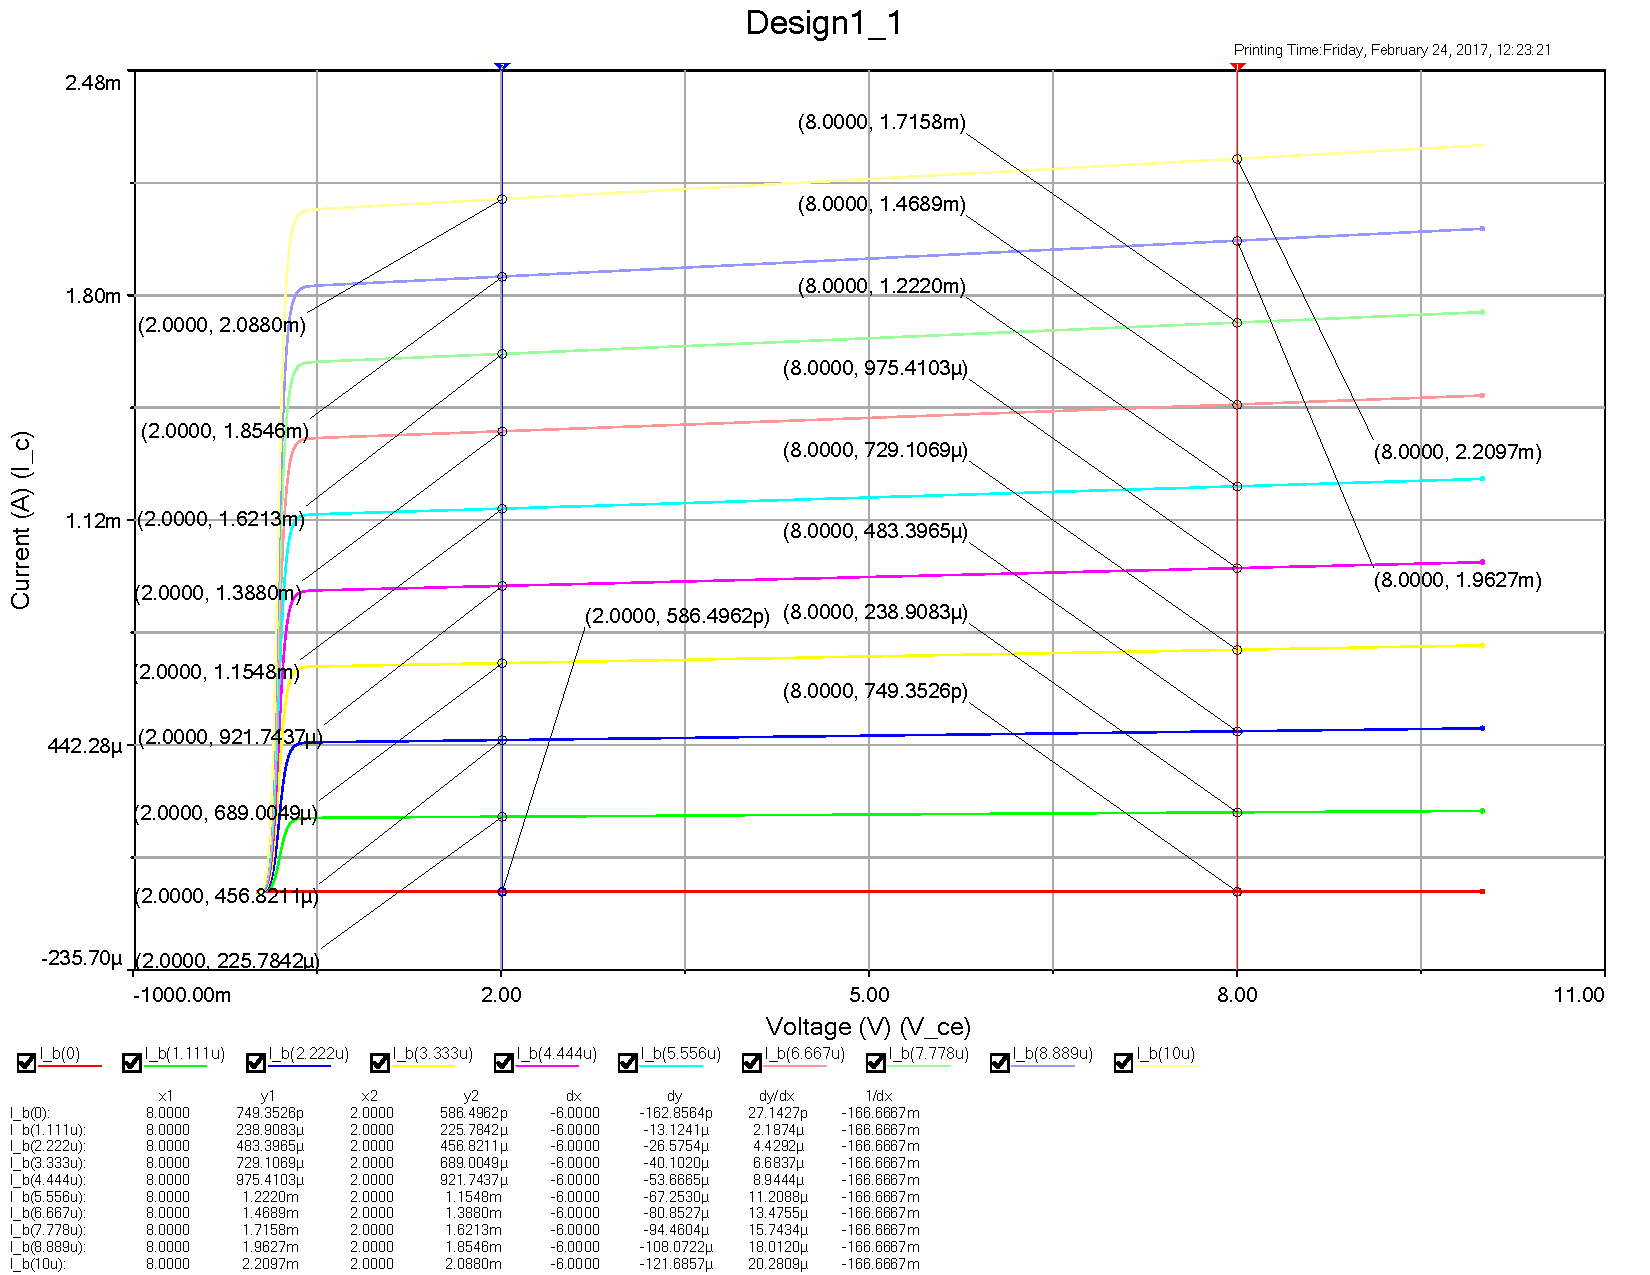
\includepdf[width=\textwidth]{T1fewf.pdf}
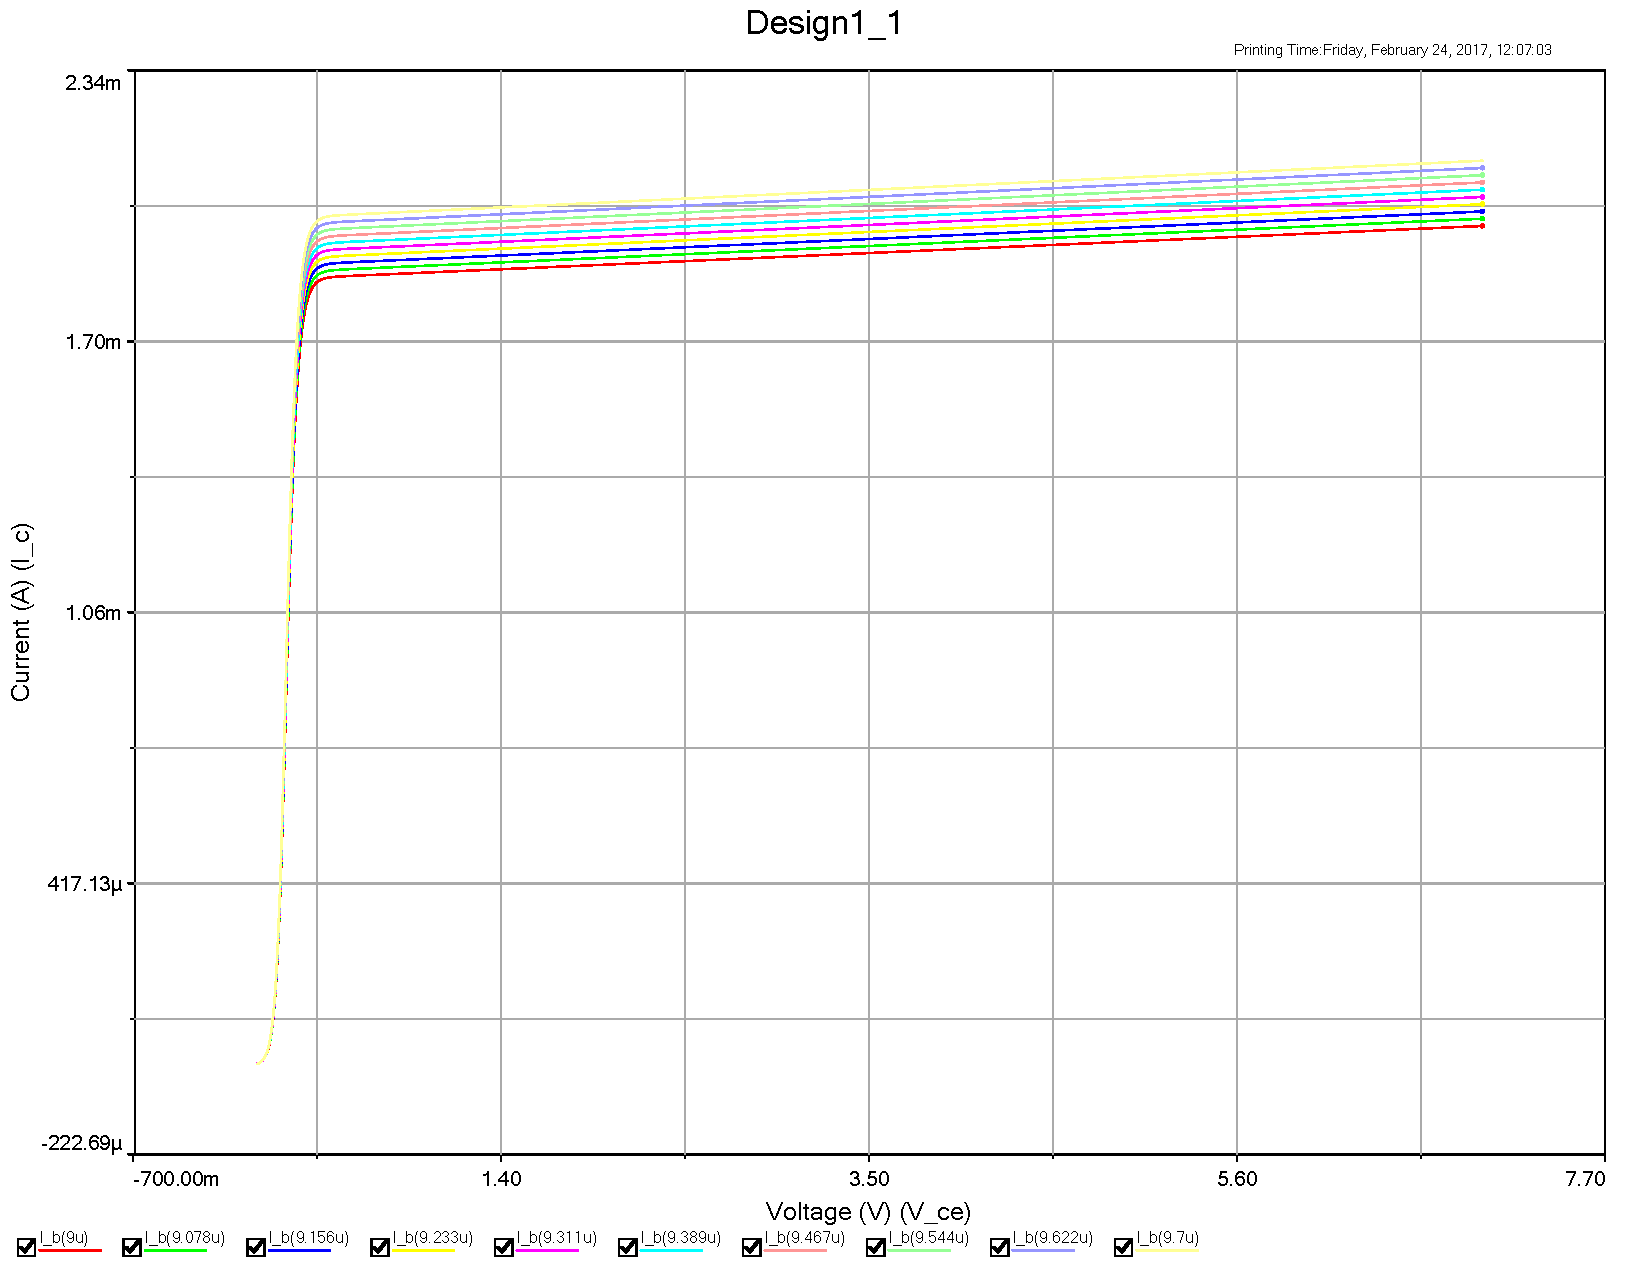
\includepdf[width=\textwidth]{1Tmicro.pdf}
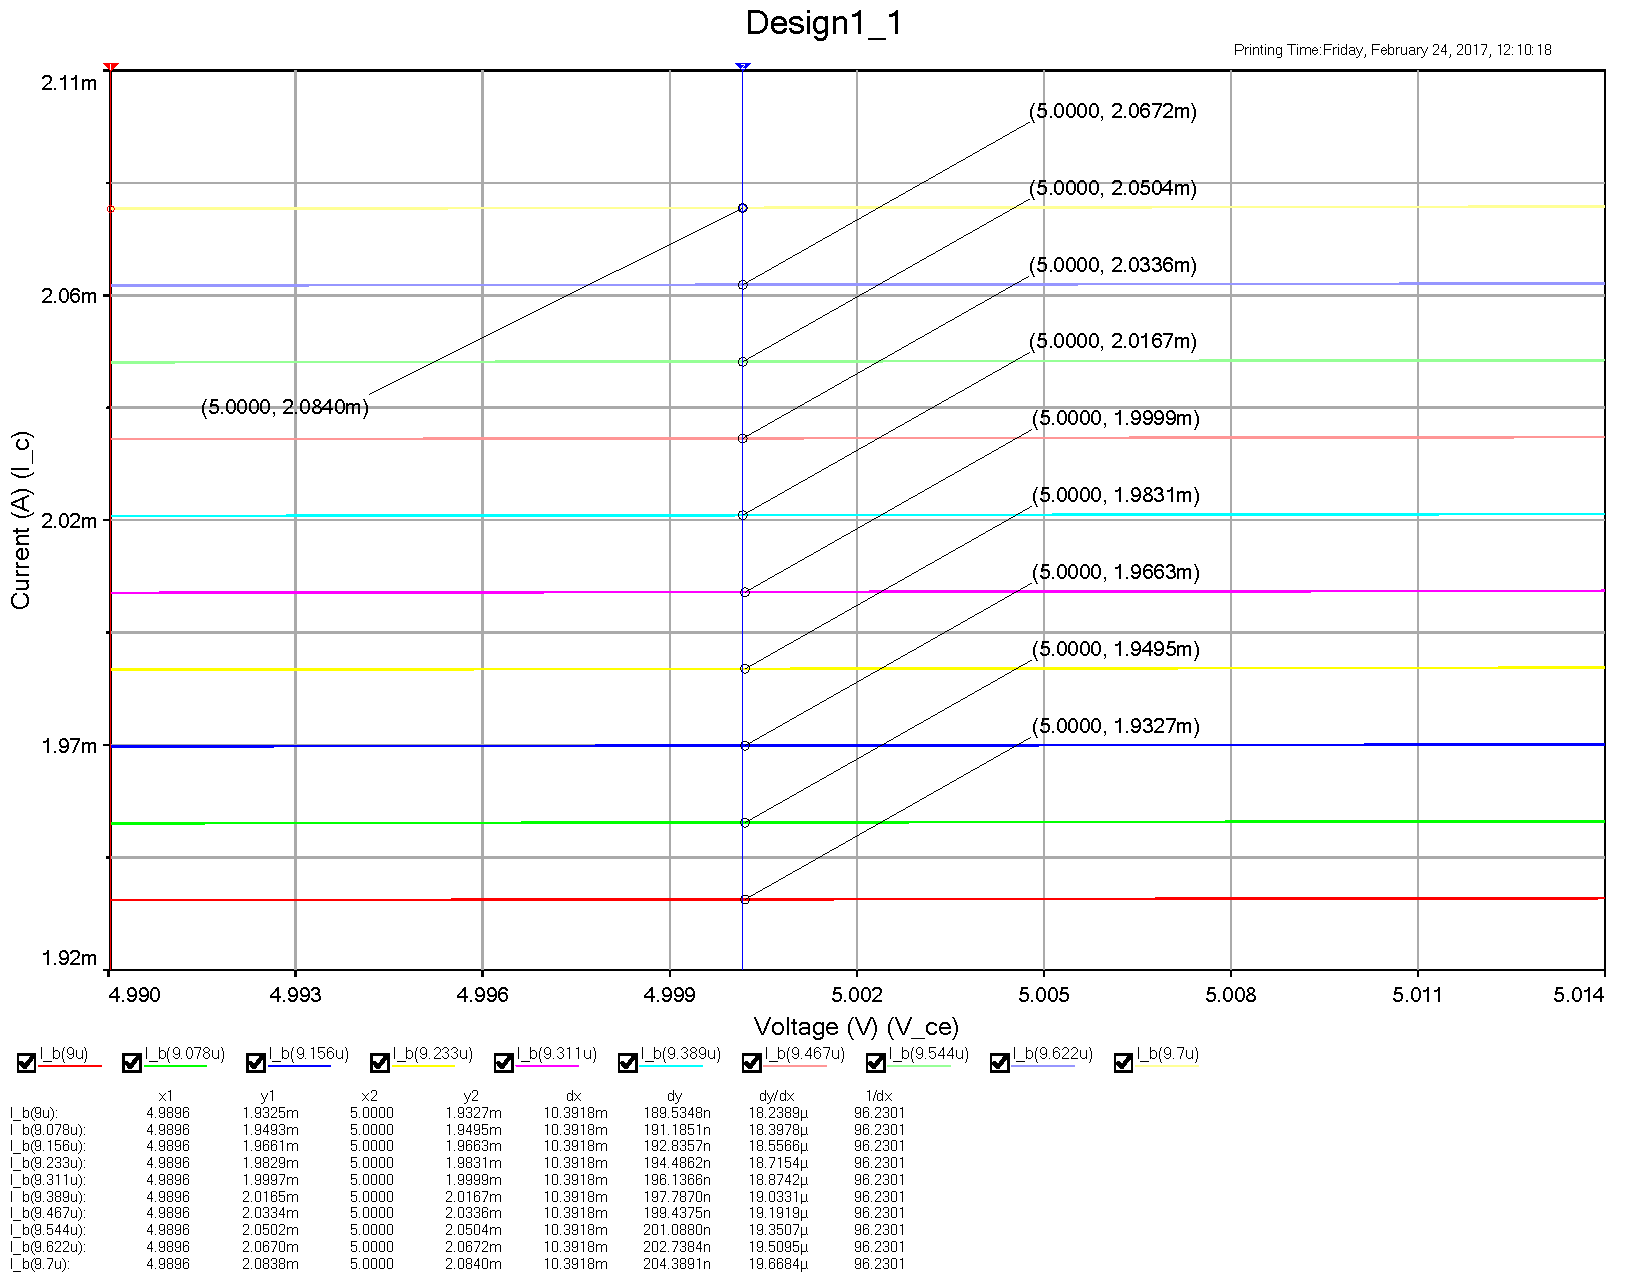
\includepdf[width=\textwidth]{5V200m1T.pdf}

\section{}
\subsection{}
\begin {wrapfigure}{r}{0pt}
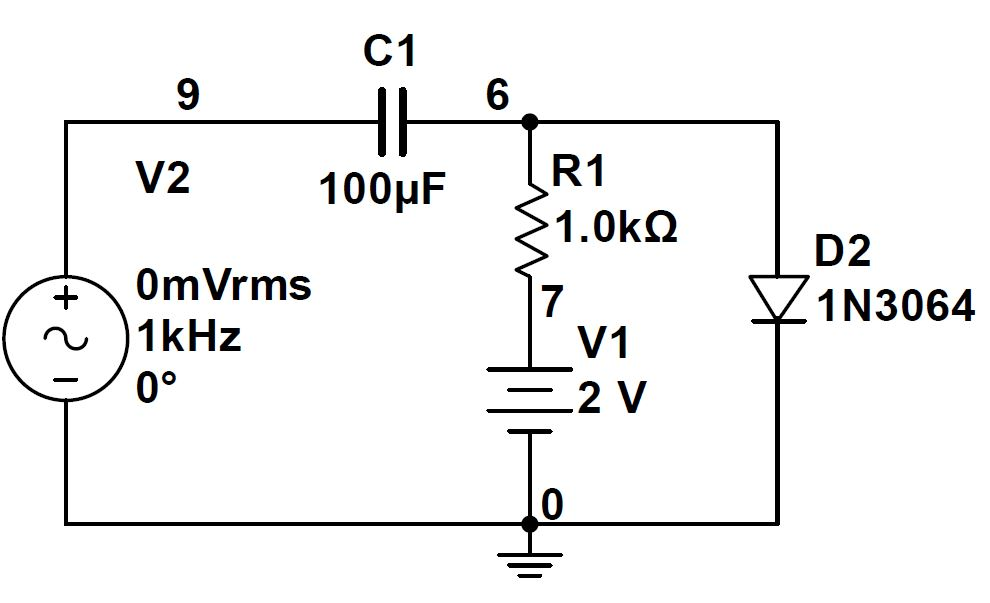
\includegraphics [width=40mm]{cap/10.JPG}
\end {wrapfigure}
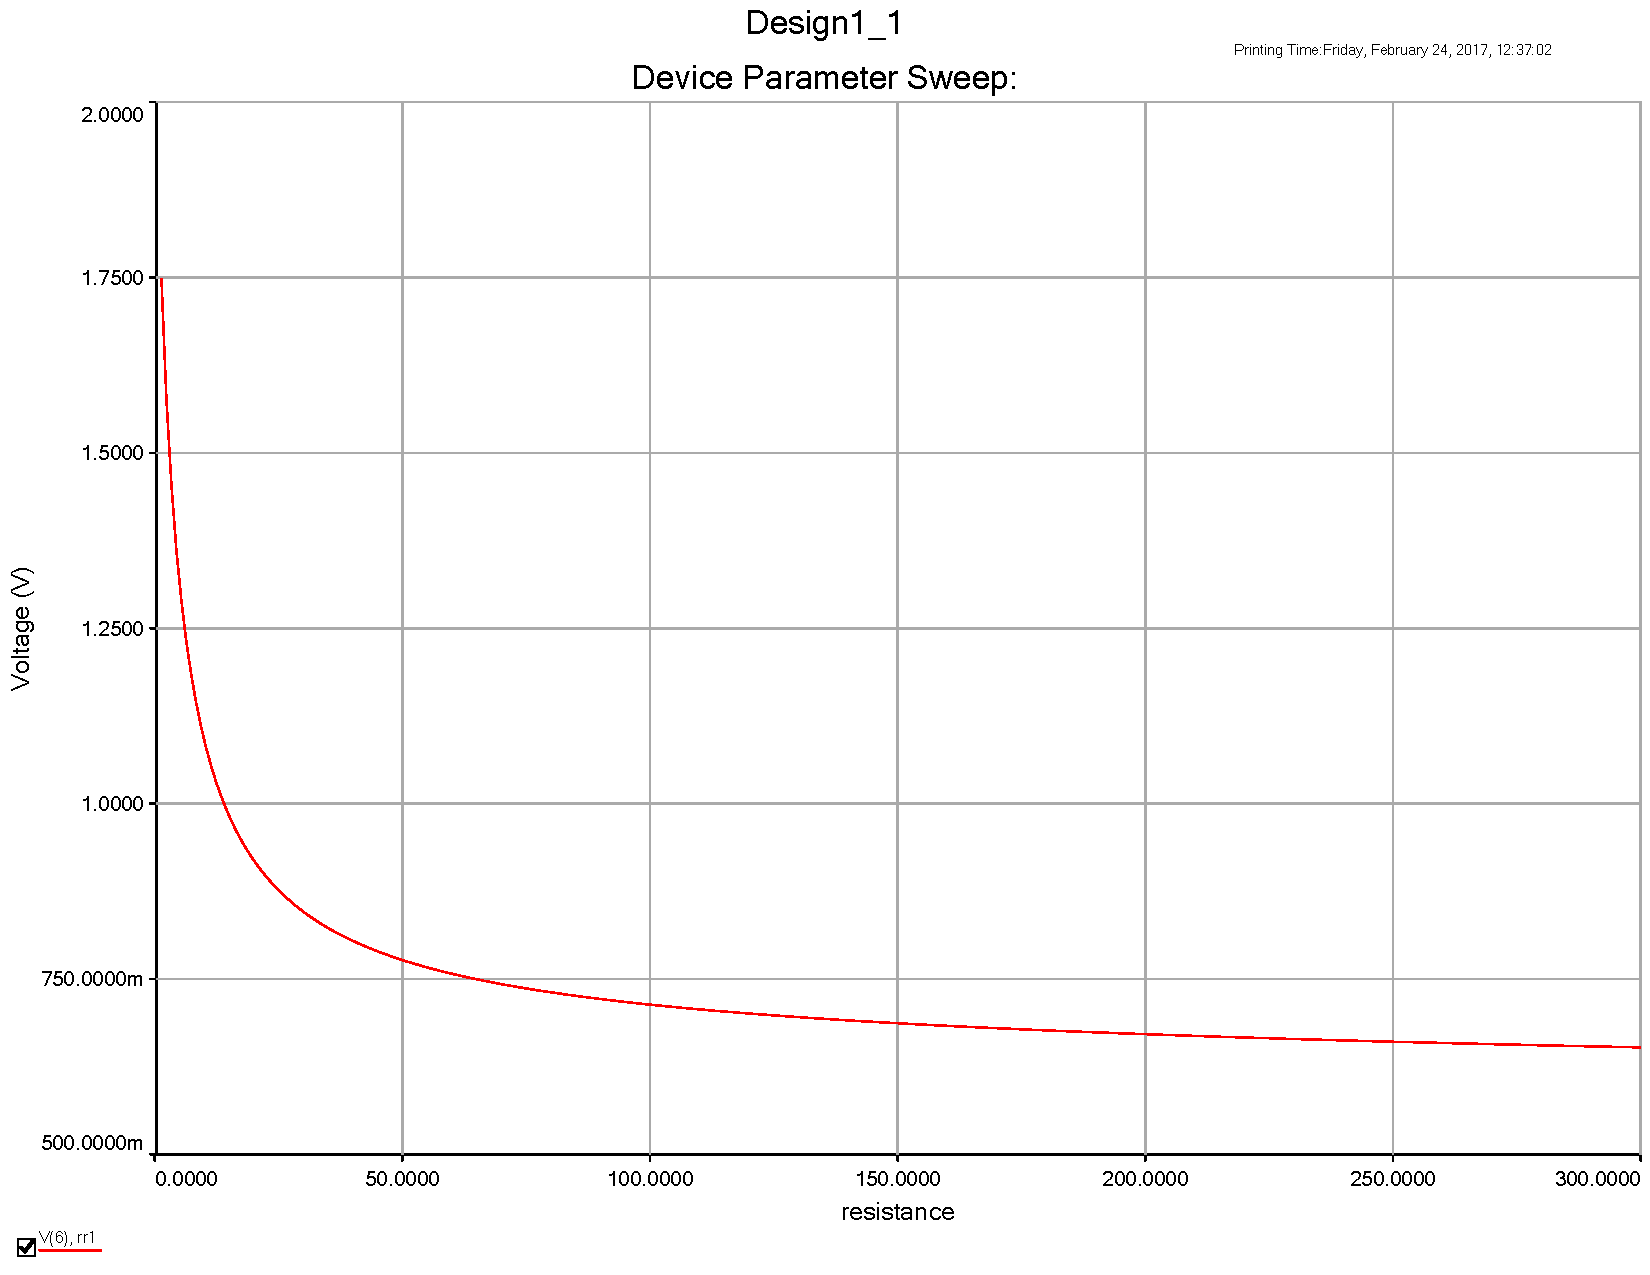
\includepdf[width=\textwidth]{3D3.pdf}
\begin {wrapfigure}{r}{0pt}
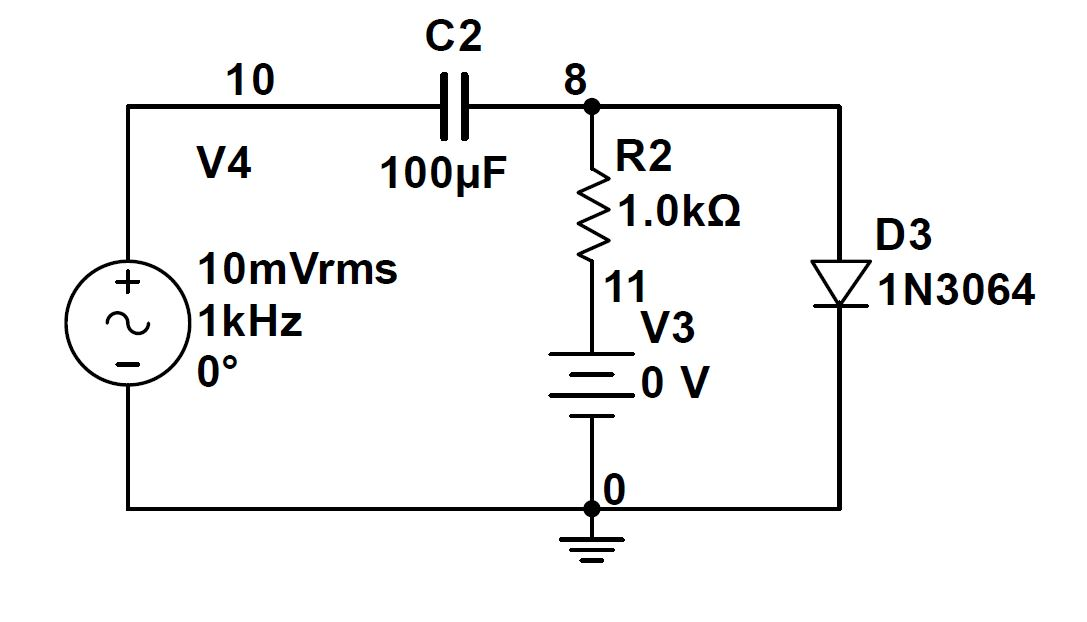
\includegraphics [width=40mm]{cap/11.JPG}
\end {wrapfigure}
\section{}
\begin {wrapfigure}{r}{0pt}
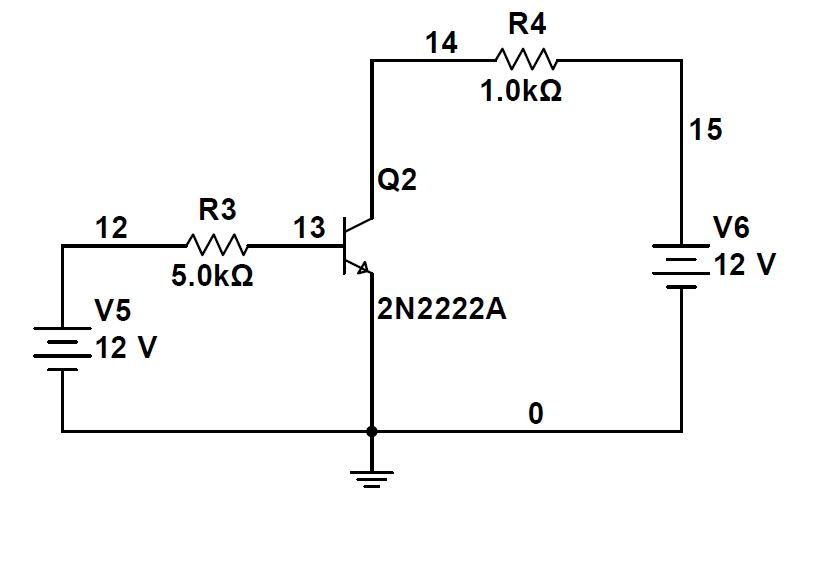
\includegraphics [width=40mm]{cap/12.JPG}
\end {wrapfigure}
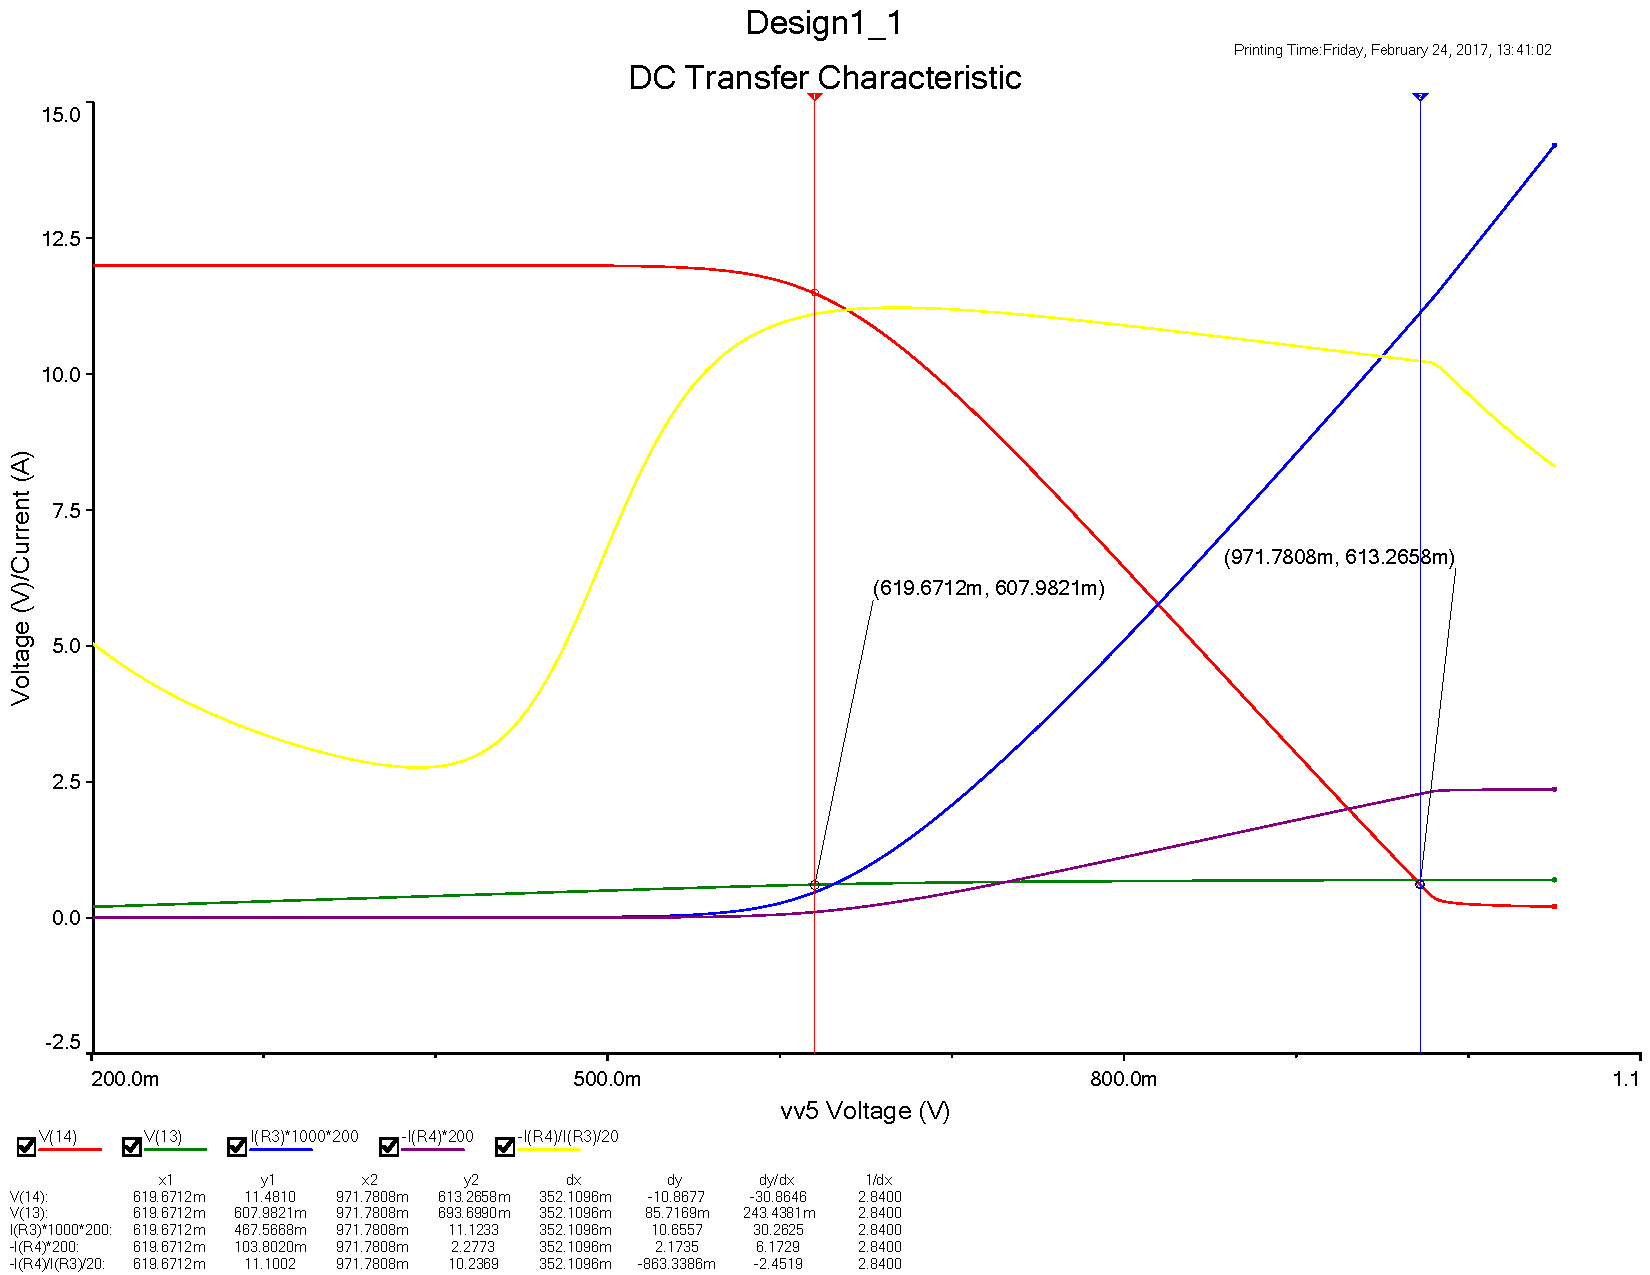
\includepdf[width=\textwidth]{efefe.pdf}
\end {document}
